\newpage
%%%%%%%%%%%%%%%%%%%%%%%%%%%%%%%%%%%%%%%%%%%%%%%%%%%%%%%%%%%%%%%%%%%%%%%%%%%%%%%%%%%%%%%%%%%%%%%%%%%%%%%%%%%%%%%%%%%%%
\section{Objetivo}
El objetivo del presente proyecto es definir y justificar los datos y características constructivas y técnicas necesarios para la realización de la instalación eléctrica automatización de una fábrica de complementos alimenticios, exponiendo ante los organismos competentes que la instalación que nos ocupa reúne las condiciones y garantías exigidas por la reglamentación vigente, a fin de obtener la Autorización Administrativa y la de Ejecución de la instalación por parte de la Dirección General de Industria, Energía y Minas, Gobierno de la Comunidad de Madrid y Ayuntamiento de Rivas-Vaciamadrid.\
 
%%%%%%%%%%%%%%%%%%%%%%%%%%%%%%%%%%%%%%%%%%%%%%%%%%%%%%%%%%%%%%%%%%%%%%%%%%%%%%%%%%%%%%%%%%%%%%%%%%%%%%%%%%%%%%%%%%%%%
\section{Ubicacion}

La Instalación objeto del presente proyecto se realizará en una nave industrial de $1620m^2$ de superficie útil construida en el año 1992 ubicada en la siguiente dirección:\\

 {\bfseries Calle de la Fundición 8, Rivas-Vaciamadrid, Comunidad de Madrid, (España)}

%%%%%%%%%%%%%%%%%%%%%%%%%%%%%%%%%%%%%%%%%%%%%%%%%%%%%%%%%%%%%%%%%%%%%%%%%%%%%%%%%%%%%%%%%%%%%%%%%%%%%%%%%%%%%%%%%%%%%
\section{Antecedentes}

La nave industrial en la cual se realizará la instalación objeto de este proyecto estuvo ocupada por un concesionario y taller de reparación de automóviles desde el año 1992 hasta el año 2013. La propiedad adquirió la nave industrial en el año 2013 con el objetivo de reconvertir el espacio en una fábrica de complementos alimenticios, dada la fuerte demanda que está teniendo este tipo de productos en los últimos años. Las instalaciones eléctricas de se desmantelaron para la reconversión, siendo su diseño parte del objeto del presente proyecto.\

%%%%%%%%%%%%%%%%%%%%%%%%%%%%%%%%%%%%%%%%%%%%%%%%%%%%%%%%%%%%%%%%%%%%%%%%%%%%%%%%%%%%%%%%%%%%%%%%%%%%%%%%%%%%%%%%%%%%%
\section{Normativa}

En el estudio y redacción del siguiente proyecto se han tenido en cuenta las siguientes normas y reglamentos actualmente en vigor:\\

{\bfseries Ley 54/1997 de 27 de Noviembre, de Regulación del Sector Eléctrico} (B.O.E. 28 de Noviembre de 1997).\\

{\bfseries Real Decreto 1995/2000}, de 1 de diciembre, por el que se regulan las actividades de transporte, distribución, comercialización, suministro y procedimientos de autorización de instalaciones de energía eléctrica.\\

{\bfseries Reglamento Electrotécnico para Baja Tensión. (R.E.B.T.)}\
Real Decreto 842/2002 de 2 de agosto.\\

{\bfseries Orden de 13-03-2002 de la Consejería de Industria y Trabajo}, por la que se establece el contenido mínimo en proyectos de industrias y de instalaciones Industriales.\\

{\bfseries Código Técnico de la Edificación.} (C.T.E.) Real Decreto 314/2006, de 17 de marzo.\\

{\bfseries Normas UNE, UNE-EN, EN e IEC}\\

{\bfseries Normas particulares de la Compañía Suministradora.}\\

{\bfseries Ordenanzas Municipales del Ayuntamiento de Rivas-Vaciamadrid.}\\

{\bfseries Directiva 2002/46/CE} del Parlamento Europeo y del Consejo, de 10 de junio de 2002, relativa a la aproximación de las legislaciones de los Estados miembros en materia de complementos alimenticios.\\

{\bfseries Reglamento (CE) 1137/2008} del Parlamento Europeo y del Consejo, de 22 de octubre de 2008 , por el que se adaptan a la Decisión 1999/468/CE del Consejo determinados actos sujetos al procedimiento establecido en el artículo 251 del Tratado, en lo que se refiere al procedimiento de reglamentación con control.\\

{\bfseries Reglamento (CE) n o 1170/2009} de la Comisión, de 30 de noviembre de 2009 , por la que se modifican la Directiva 2002/46/CE del Parlamento Europeo y del Consejo y el Reglamento (CE) n o 1925/2006 del Parlamento Europeo y del Consejo en lo relativo a las listas de vitaminas y minerales y sus formas que pueden añadirse a los alimentos, incluidos los complementos alimenticios.\\

{\bfseries Real Decreto 1487/2009}, de 26 de septiembre, relativo a los complementos
alimenticios.\\

{\bfseries Otros reglamentos vigentes que le sean de aplicación.}\\

En caso de producirse alguna diferencia de criterio entre una normativa y otra debe permanecer la de rango superior, siempre y cuando la de rango inferior no fuese más perceptiva.

%%%%%%%%%%%%%%%%%%%%%%%%%%%%%%%%%%%%%%%%%%%%%%%%%%%%%%%%%%%%%%%%%%%%%%%%%%%%%%%%%%%%%%%%%%%%%%%%%%%%%%%%%%%%%%%%%%%%%
\section{Descripción general}

La nave industrial se divide de dos áreas diferenciadas: un zona de oficinas de dos plantas con una superficie útil por planta de 175$m^2$ y la zona industrial con una superficie útil de 1260$m^2$, siendo la superficie total 1610${m^2}$. La zona industrial se divide en tres zonas: zona de carga y descarga, zona de almacenamiento de materia prima, zona de almacenamiento del producto y zona de fabricación. La zona de oficinas consta de una recepción, una zona de oficina por planta, zona de personal de fábrica y vestuarios, centro de control y una zona de aseos por planta.
\\

Los camiones entrarían marcha atrás en la nave y los empleados procederían a descargar su contenido con la ayuda de carretillas elevadoras. Los palets con los sacos con la materia prima en polvo, así como los de los cartones para ensamblar las cajas se almacenarían en estanterías de palets situadas en la zona de almacenamiento de materia prima. 
\\

En la zona de fabricación se llevará a cabo todo el proceso de transformación del polvo a pastillas envasadas en cajas. Se situarán un horno de secado, una máquina de compresión, una máquina de verificación, un tambor de revestimiento, una máquina de formación de blisters y una última de embalaje, así como cintas para transportar los distintos elementos y dos brazos robóticos para paletizar el producto final. Estos palets se almacenan en estanterías cerca de la puerta en la zona de almacenamiento de producto.\\

Las máquinas de la zona de fabricación disponen de una serie de sensores y actuadores que serán controlados por PC Industrial a través de una tarjeta de adquisición de datos. Se realizará tanto la instalación física de las máquinas, su electrificación y control, como la instalación eléctrica de la zona de oficinas y zona industrial. Todos los detalles y características de los elementos y procesos se encuentran detallados en las siguientes secciones del presente documento.

%%%%%%%%%%%%%%%%%%%%%%%%%%%%%%%%%%%%%%%%%%%%%%%%%%%%%%%%%%%%%%%%%%%%%%%%%%%%%%%%%%%%%%%%%%%%%%%%%%%%%%%%%%%%%%%%%%% 
\section{Elementos del sistema}

\subsection{Instalación eléctrica}

\subsubsection{Red de suministro}

La empresa encargada de suministrar energía eléctrica a la instalación será UNIÓN FENOSA, S.A.\\

Características de la red de suministro:\

\begin{itemize}
\item {\bfseries Red:} Corriente Alterna Trifásica 
\item {\bfseries Tensión:} 400/230V (Entre fases y entre fase y neutro)
\item {\bfseries Frecuencia:} 50 Hz
\item {\bfseries Intensidad de cortocircuito trifásico:} 12 kA
\end{itemize}

El suministro se realizará a través de {\bfseries Acometida Subterránea con conductores unipolares de aluminio RV 0,6/1kV 3x240+1x150 Al} instalados bajo tubo enterrado, llegando a una CGP de instalación empotrada. La instalación será existente, siendo sólo objeto de este proyecto la instalación aguas abajo a partir del Cuadro General de Mando y Protección cuya envolvente se ajusta a las normas UNE 20.451 y UNE-EN 60.439 -3, con un grado de protección IP 30 según UNE 20.324 e IK07 según UNE-EN 50.102.\\

Para la sección de conductores indicada previamente, teniendo en cuenta sus características de instalación existente y que los fusibles instalados en la CGP son de 350A, se establece una {\bfseries potencia máxima admisible en la instalación de 243kW}

\subsubsection{Previsión de potencia}

La potencia total prevista para la instalación, usada para el cálculo del interruptor automático general se obtendrá, teniendo en cuenta los interruptores automáticos del cuadro general de mando y protección y un factor de corrección por simultaneidad 0,7:

$$P_{total}=\left( \sum \sqrt 3 \cdot I_{automatico\ i}\cdot  {V_{linea}}\right)\cdot 0,7$$\

Se obtiene un valor de {\bfseries potencia total de 222kW}\\

Para el cálculo la previsión de potencia de cada circuito se multiplicará la potencia nominal demandada por cada receptor por el número de receptores a instalar. Para circuito de las cintas transportadoras se aplicará un factor de corrección de 1,5 a la potencia total. Para el resto de receptores el factor de corrección será 1. \\

La previsión de potencia de cada circuito, así como el número de receptores a instalar y su distribución en los cuadros se encuentran detallados en el apartado [PLANOS]. Los cálculos se encuentran detallados en el apartado [CALCULOS]. 

\subsubsection{Cuadro General de Mando y Protección y cuadros secundarios}

La instalación eléctrica partirá del Cuadro General de Mando y Protección y se distribuirá entre dos cuadros secundarios como se detalla en el [ANEXO PLANOS!!]. La envolvente del Cuadro General de Mando y Protección es existente y se reutilizará de la instalación anterior. Las envolventes de los cuadros secundarios serán de [CARACTERíSTICAS], como viene detallado en el apartado [PRESUPUESTO!!]\\

Los dispositivos generales e individuales de mando y protección de serán, como mínimo: un Interruptor general automático de corte omnipolar por cuadro, que permita su accionamiento manual y que esté dotado de elementos de protección contra sobrecarga y cortocircuitos, interruptores automáticos individuales para cada circuito con las mismas características que el interruptor general automático y un interruptor diferencial por cada 5 circuitos como mínimo. La sensibilidad de los interruptores diferenciales responderá a lo señalado en la Instrucción ITC-BT-24. Todas los Interruptores Automáticos Magnetotérmicos serán de corte omnipolar, tipo de curva C y poseerán un poder de corte de 6 kA. Se seleccionarán protecciones con un poder de corte de 6 kA al ser más económicos que los de poder de corte 4,5 kA que se exigen como mínimo por normativa.\\

La elección calibre de las protecciones de los interruptores automáticos individuales vendrá determinada por la potencia máxima demandada por cada receptor y la intensidad máxima admisible por los conductores que lo alimentan, siguiendo el criterio:\

$$ I_{MAX\ demandada\ receptor}\leq I_{AUTOMATICO}\leq I_{MAX\ admisible\ conductores}$$

La distribución de los cuadros, así como los calibres de las protecciones y los circuitos a los que alimentan se encuentra detallado en el apartado [PLANOS]. Los cálculos de los calibres de los interruptores automáticos vendrán justificados en el apartado [CALCULOS]

\subsubsection{Instalación eléctrica de la oficina}

Es la parte de la instalación eléctrica que partiendo del cuadro de de la oficina, enlaza con los receptores de iluminación, tomas de corriente de uso general, tomas de corriente de baño y tomas de corriente SAI.\\

Está regulada en las ITC-BT 25 e ITC-BT 26 del R.E.B.T. donde se especifican las prescripciones generales de instalación y calibres de los tubos a utilizar en cada circuito. Los conductores utilizados para estos circuitos serán de cobre unipolares con aislamiento de cobre y una tensión asignada de 450/750V (H07Z1-K) siendo no propagadores del incendio y con emisión de humos y opacidad reducida. La instalación de estos conductores realizará bajo tubo curvable de 2 capas en montaje empotrado en pared de mampostería o bajo falso techo, donde proceda.\\

La elección de las secciones de los conductores vendrá determinada por la potencia máxima demandada por cada receptor y la intensidad máxima admisible por los conductores que lo alimentan, siguiendo siguiendo los siguientes criterios:\\

{\bfseries Criterio de caída de tensión}

La caída de tensión sera como máximo del 3\% en los circuitos de alumbrado y un 5\% en el resto de instalaciones. Esta caída de tensión se calculará para una intensidad de funcionamiento del circuito igual a la intensidad nominal del interruptor automático de dicho circuito y para una distancia correspondiente a la del punto de utilización mas alejado del origen de la instalación. El valor de la caída de tensión podrá compensarse entre el de la instalación eléctrica de la oficina y el de la derivación del Cuadro General de Mando y Protección al cuadro de la oficina, de forma que la caída de tensión total sea inferior a la suma de los valores límite especificados para ambas. Se calculará usando las siguientes fórmulas:\\

Para circuitos de corriente alterna monofásica:\\

$$ S=\frac{2\cdot \rho \cdot L_o	\cdot I\cdot cos(\varphi)}{\Delta V}$$

Para circuitos de corriente alterna trifásica:\\

$$ S=\frac{\sqrt{3} \cdot \rho \cdot L_o \cdot I\cdot cos(\varphi)}{\Delta V}$$

Siendo $\Delta V$ la caída de tensión en voltios, $cos(\varphi)$ el factor de potencia activa, $L$ la longitud del cable en metros y $\rho$ la resistividad del conductor en $\Omega mm^2$


{\bfseries Criterio de Intensidad máxima admisible}

Las Intensidades Máximas Admisibles de los conductores se regirán en su totalidad por lo indicado en la norma UNE 20460-5-523.

{\bfseries Criterio de Intensidad de cortocircuito}

Se regirán en su totalidad por lo indicado en la ITC-BT 17. Se toma el defecto fase-neutro como el más desfavorable y se considera despreciable la reactancia inductiva de los conductores. La resistencia de los conductores para el cálculo será a 20 ºC 

Las instalación eléctrica de la oficina, al tratarse de un lugar de pública concurrencia y local de trabajo deberá cumplir las condiciones establecidas en la ITC-BT-28: \\

\begin{itemize}
\item El cuadro general de distribución deberá colocarse en el punto más próximo posible a la entrada de la acometida o derivación individual y se colocará junto o sobre él, los dispositivos de mando y protección establecidos en la instrucción ITC-BT-17. Cuando no sea posible la instalación del cuadro general en este punto, se instalará en dicho punto un dispositivo de mando y protección.\\

\item Del citado cuadro general saldrán las líneas que alimentan directamente los aparatos receptores o bien las líneas generales de distribución a las que se conectará mediante cajas o a través de cuadros secundarios de distribución los distintos circuitos alimentadores. Los aparatos receptores que consuman más de 16 amperios se alimentarán directamente desde el cuadro general o desde los secundarios.

\item El cuadro general de distribución e, igualmente, los cuadros secundarios, se instalarán en locales lugares o recintos a los que no tenga acceso el público y que estarán separados de los locales donde exista un peligro acusado de incendio o de pánico (cabinas de proyección, escenarios, salas de público, escaparates, etc.), por medio de elementos a prueba de incendios y puertas no propagadoras del fuego. Los contadores podrán instalarse en otro lugar, de acuerdo con la empresa distribuidora de energía eléctrica, y siempre antes del cuadro general.

\item En el cuadro general de distribución o en los secundarios se dispondrán dispositivos de mando y protección contra sobreintensidades, cortocircuitos y contactos indirectos para cada una de las líneas generales de distribución, y las de alimentación directa a receptores. Cerca de cada uno de los interruptores del cuadro se colocará una placa indicadora del circuito al que pertenecen.

\item En las instalaciones para alumbrado de locales o dependencias donde se reúna público, el número de líneas secundarias y su disposición en relación con el total de lámparas lámparas a alimentar, deberá ser tal que el corte de corriente en una cualquiera de ellas no afecte a más de la tercera parte del total de lámparas lámparas instaladas en los locales o dependencias que se iluminan alimentadas por dichas líneas. Cada una de estas líneas estarán protegidas en su origen contra sobrecargas, cortocircuitos, y si procede contra contactos indirectos.

\end{itemize}

Las canalizaciones serán de tubo corrugado para el montaje empotrado. Estos tipos de tubos serán antiinflamables y por tanto, no propagadores de la llama. Los angulos de curvatura no serán en ningún momento inferiores a 90, con el fin de permitir el acceso a los conductores. Las canalizaciones deben realizarse según lo dispuesto en las ITC-BT-19 e ITC-BT-20 y estaran constituidas por:

\begin{itemize}
\item Conductores aislados, de tensión nominal no inferior a 450/750 V, colocados bajo tubos o canales protectores, preferentemente empotrados en especial en las zonas accesibles al público.

\item Conductores aislados, de tensión nominal no inferior a 450/750 V, con cubierta de protección, colocados en huecos de la construcción, totalmente construidos en materiales incombustibles de grado de resistencia al fuego incendio RF-120, como mínimo.

\item Los cables y sistemas de conducción de cables deben instalarse de manera que no se reduzcan las características de la estructura del edificio en la seguridad contra incendios.

\item Los cables eléctricos a utilizar en las instalaciones de tipo general y en el conexionado interior de cuadros eléctricos en este tipo de locales, tendrán propiedades especiales frente al fuego, siendo no propagadores del incendio y con emisión de humos y opacidad reducida. Los cables con características equivalentes a la norma UNE 21.123, partes 4 ó 5, o a la norma UNE 211002 (según la tensión asignada del cable) cumplen con esta prescripción.

\item Los cables eléctricos a utilizar en las instalaciones de tipo general y en el conexionado interior de cuadros eléctricos en este tipo de locales, serán no propagadores del incendio y con emisión de humos y opacidad reducida. Los cables con características equivalentes a las de la norma UNE 21.123 parte 4 ó 5; o a la norma UNE 211002 (según la tensión asignada del cable), cumplen con esta prescripción.

\item Los elementos de conducción de cables con características equivalentes a los clasificados como "no propagadores de la llama" de acuerdo con las normas UNE-EN 50085-1 y UNE-EN 50086-1, cumplen con esta prescripción.

\item Los cables eléctricos destinados a circuitos de servicios de seguridad no autónomos o a circuitos de servicios con fuentes autónomas centralizadas, deben mantener el servicio durante y después del incendio, siendo conformes a las especificaciones de la norma UNE-EN 50.200 y tendrán emisión de humos y gases tóxicos muy opacidad reducida. Los cables con características equivalentes a la norma UNE 21.123, apartado 3.4.6, cumplen con esta prescripción de emisión de humos y opacidad reducida.

\end{itemize}

Los conductores de la instalación deben ser fácilmente identificados, especialmente por lo que respecta a los conductores neutro y de protección. Esta identificación se realizará por los colores que presenten sus aislamientos. Cuando exista conductor neutro en la instalación o se prevea para un conductor de fase su pase posterior a conductor neutro, se identificarán éstos por el color azul claro. Al conductor de protección se le identificará por el doble color amarillo-verde. Todos los conductores de fase, o en su caso, aquellos para los que no se prevea su pase posterior a neutro, se identificarán por los colores marrón o negro. Solamente cuando se considere necesario identificar tres fases diferentes, podrá utilizarse el color gris.\\

En la ejecución de las instalaciones interiores de las viviendas se deberá tener en cuenta:
No se utilizará un mismo conductor neutro para varios circuitos. Todo conductor debe poder seccionarse en cualquier punto de la instalación en el que se realice una derivación del mismo, utilizando un dispositivo apropiado, tal como un borne de conexión, de forma que permita la separación completa de cada parte del circuito del resto de la instalación.\\

En ningún caso se permitirá la unión de conductores mediante conexiones y o derivaciones por simple retorcimiento o arrollamiento entre sí de los conductores, sino que deberá realizarse siempre utilizando bornes de conexión montados individualmente o constituyendo bloques o regletas de conexión. Siempre deberán realizarse en el interior de cajas de empalme y / o derivación (Según ITC-BT 19).\\

Los materiales seleccionados para los circuitos de la zona de oficinas serán:

Tomas de Corriente C2a (Schuko): BJC Serie Iris (Blanco) o superior.

Mecanismos (Interruptores): BJC Serie Iris sin difusor (Blanco) o superior.

Iluminación incandescente: Lámparas halógenas Phillips Fugato o superiores.

Iuminación fluorescente: Luminarias fluorescentes Phillips M2-BD45 o equivalentes.

La distribución de los circuitos así como las secciones de los conductores a instalar aparecen reflejados en el apartado [PLANOS] del presente proyecto. Los cálculos de las secciones de los conductores vendrán justificados en el apartado [CALCULOS]

\subsubsection{Instalación elécrtica de la zona de fabricación y almacén}

Las canalizaciones seran de tubo de PVC curvable en caliente para lo que se instale superficialmente, admitiendose tubo corrugado para el montaje empotrado. Estos tipos de tubos seran antiinflamables y por tanto, no propagadores de la llama.
Los ángulos de curvatura no seran en ningún momento inferiores a 90 grados, a fin de permitir el acceso a los conductores.
Para determinar el diámetro de los tubos a emplear en función de los mismos que ha de alojar, se han de emplear las tablas de la Instrucción ITC-BT-21.




altura de las luminarias, tomas de maquinas, bandejas

altura d elas tomas mecanismos tubos de aluminio



\subsection{Maquinaria}
	\subsubsection{Máquina de secado de polvo}
	\subsubsection{Máquina de compresión en tabletas}
	\subsubsection{Máquina de verificación de dureza de tabletas}
	\subsubsection{Máquina de revestimiento de tabletas}
	\subsubsection{Máquina de sellado de blisters }
	
	\subsubsection{Máquina de empaquetado}
	\subsubsection{Robot de paletizado}
%%%%%%%%%%%%%%%%%%%%%%%%%%%%%%%%%%%%%%%%%%%%%%%%%%%%%%%%%%%%%%%%%%%%%%%%%%%%%%%%%%%%%%%%%%%%%%%%%%%%%%%%%%%%%%%%%%%%%	
\section{Sistema propuesto}


Cuando el horno emita una señal de aviso un operario procederá a llenar el depósito de dicho horno con la materia prima. Una vez lleno, el horno libera el polvo uniformemente sobre una cinta transportadora. Esta lo transporta por el horno de manera ondulante para eliminar cualquier tipo de humedad. 
\\

A la salida del horno el polvo es introducido en una máquina de compresión, donde es convertido en pastillas y se le imprime el nombre de la pastilla.  Acto seguido pasa por una máquina de comprobación, que desecha cualquier pastilla que haya resultado demasiado frágil por seguir húmeda tras el horno. Las pastillas desechadas, se trituran y depositan en un recipiente para que el operario lo reintroduzca en el horno en la siguiente iteración. 
\\

El resto de pastillas continúa hasta un tambor donde se les da un revestimiento de agua con colorantes para su identificación y conservación, al endurecer así la capa exterior y evitar que se deshagan. Tras ser rociadas por pulsos muy rápidos y cortos para favorecer un secado rápido son transportadas a una máquina de sellado.
\\

En esta máquina se dejan caer pastillas hasta llenar un depósito, donde mediante un sensor indica el llenado. La selladora coloca las pastillas en posición segun la matriz utilizada. Paralelamente tira del rollo de plástico en lámina y lo coloca debajo de la parte superior. Al bajar, ésta deforma la lámina con unos cabezales calientes y crea los habitáculos donde inmediatamente inserta las tabletas. Acto seguido se corta el plástico y este avanza a la siguiente posición donde se le coloca una lámina de alumnio con el logo impreso y es sellado por calor al bajar la parte superior en la siguiente iteración. 
\\

Finalmente se transportan los blisters sellados por otra cinta transportadora a la máquina de empaquetado, que coge las cartulinas de las cajas y las dobla para darles su forma final e inserta los blisters en la caja, asi como un folleto explicativo previamente impreso y doblado. Las cajas con el produto final se dejan caer por una rampa hasta una mesa donde un brazo robótico equipado con una cámara coge las cajas individuales y las coloca en cajas de lotes en un palé para ser recogido por un operario y almacenado en una estantería. Un segundo brazo robótico coje un palé de una pila de palés vacíos y lo coloca en la posición del anterior.
\\
%%%%%%%%%%%%%%%%%%%%%%%%%%%%%%%%%%%%%%%%%%%%%%%%%%%%%%%%%%%%%%%%%%%%%%%%%%%%%%%%%%%%%%%%%%%%%%%%%%%%%%%%%%%%%%%%%%%%%
\section{Flujograma}
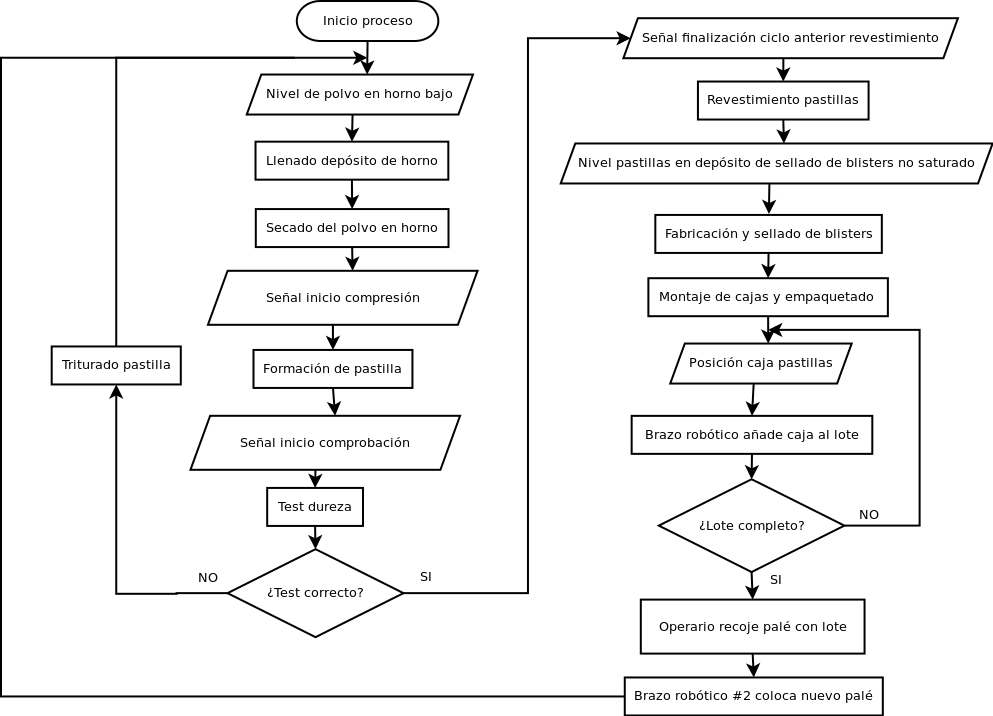
\includegraphics[width=15cm,height=20cm,keepaspectratio]{Planos/Flujograma.png}



%%%%%%%%%%%%%%%%%%%%%%%%%%%%%%%%%%%%%%%%%%%%%%%%%%%%%%%%%%%%%%%%%%%%%%%%%%%%%%%%%%%%%%%%%%%%%%%%%%%%%%%%%%%%%%%%%%%%%%%%%%%%%%%%
\newpage\section {Firmas de los ingenieros}
\vspace{5cm}
Fdo. Alvaro Ferrán Cifuentes
\vspace{5cm}\hspace{5cm}
Fdo. David Antón Sánchez

%%%%%%%%%%%%%%%%%%%%%%%%%%%%%%%%%%%%%%%%%%%%%%%%%%%%%%%%%%%%%%%%%%%%%%%%%%%%%%%%%%%%%%%%%%%%%%%%%%%%%%%%%%%%%%%%%%%%%
\newpage \section{Anexos}

   
\subsection{Anexo de cálculos:}

\subsubsection{Cálculos de la Instalación eléctrica}
\paragraph{Diseño del cuadro general de protección y mando}
\paragraph{Cálculo de las líneas de alimentación de cada máquina}
\paragraph{Cálculo de las líneas para las tomas de corriente de uso general}
\paragraph{Cálculo de las líneas para las tomas de corriente con SAI}
\paragraph{Cálculo de las líneas para iluminación}
\paragraph{Cálculo de las líneas para iluminación de emergencia}

\subsubsection{Cálculo de las instalaciones de automatización}
\paragraph{Sensores }
\paragraph{Cuadro centralización de automatización}
\paragraph{Rack con PC industrial conectado a la red de la fábrica}
\subsubsection{Instalaciones de seguridad}
\paragraph{Protección de las personas}
\paragraph{Protección contra intrusión}

\subsection{Anexo de código}
\newpage
\subsection{Anexo de catálogos}
\subsubsection{Máquina de secado de polvo}
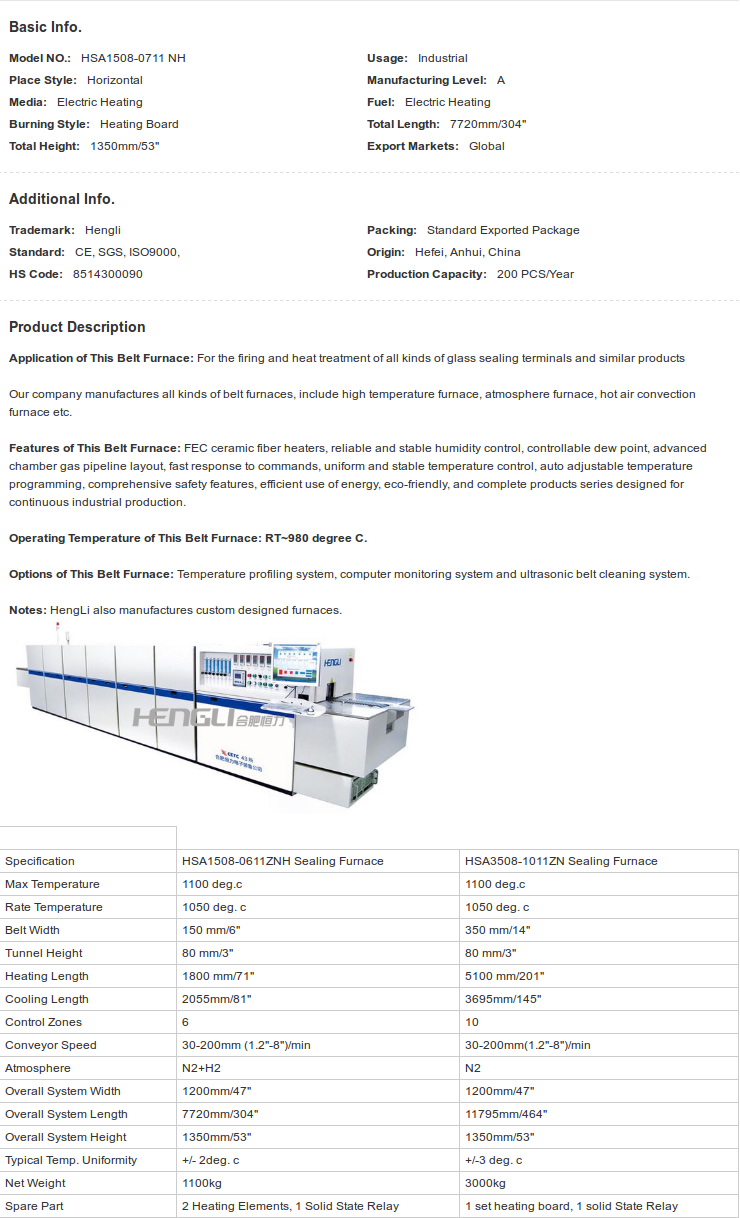
\includegraphics[width=15cm,height=20cm,keepaspectratio]{Datasheets/1Horno.png} 
\newpage

\subsubsection{Máquina de compresión en tabletas}

\includegraphics[width=15cm,height=20cm,keepaspectratio]{Datasheets/2MaquinaPrensado.png} 
\newpage

\subsubsection{Máquina de verificación de dureza de tabletas}
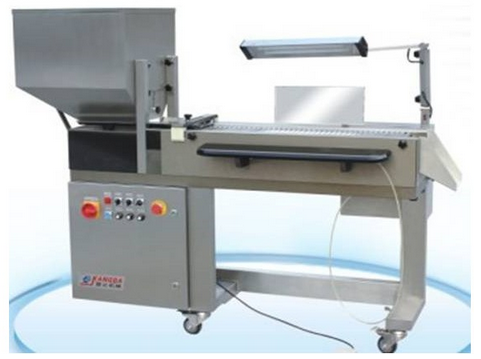
\includegraphics[width=5cm,height=4cm,keepaspectratio]{Datasheets/3Foto.png} 
\\

\includegraphics[width=15cm,height=20cm,keepaspectratio]{Datasheets/3MaquinaVerificacion.png} 
\newpage

\subsubsection{Máquina de revestimento de tabletas}
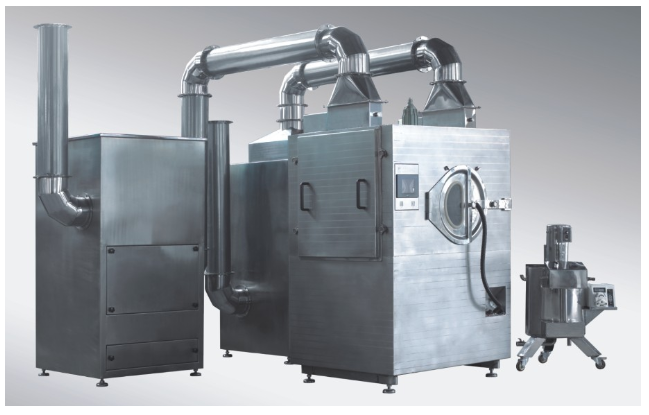
\includegraphics[width=5cm,height=4cm,keepaspectratio]{Datasheets/4Foto.png} 
\\

\includegraphics[width=15cm,height=20cm,keepaspectratio]{Datasheets/4MaquinaRevestimiento.png} 
\newpage

\subsubsection{Máquina de sellado de blisters}
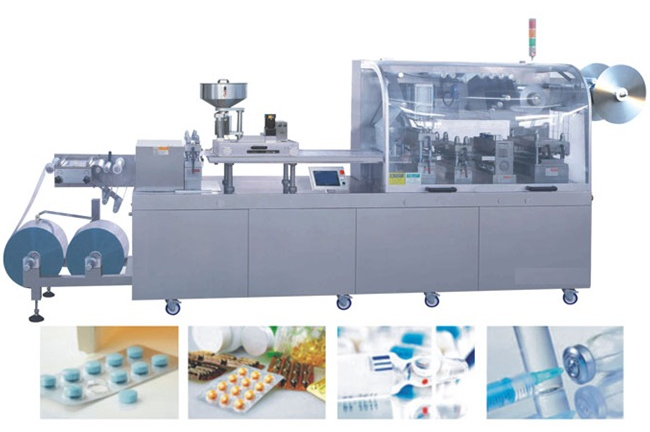
\includegraphics[width=5cm,height=4cm,keepaspectratio]{Datasheets/5Foto.png} 
\\

\includegraphics[width=15cm,height=20cm,keepaspectratio]{Datasheets/5MaquinaBlisters.png} 
\newpage

\subsubsection{Máquina de empaquetado}

\includegraphics[width=15cm,height=20cm,keepaspectratio]{Datasheets/7MaquinaEmpaquetado.png} 
\newpage
\subsubsection{Robot de paletizado}

\subsection{Planificación}

